\chapter{评价实验过程运转映射数字孪生技术研究}
\label{chap:r46-6}

本项研究围绕井筒清洁工具评价实验装置，完成三维场景构建、数字孪生应用室内部署及控制系统数据联调，实现实验运行参数监测和工具运动的虚实映射。系统将实验台架、动力驱动和流体循环装置与参数显示对应，使操作人员能够在同一界面观察工具运行状态及参数变化。

已完成装置与虚拟模型的数据联调，实现工具前进、停止、后退和旋转的映射。2026年9月30日现场画面记录了控制端与孪生端的运行参数；杭州多算科技有限公司于10月8日出具盖章的《数字孪生系统联调及参数比对情况说明》，并在附页列出参数比对和计算方法。

\section{数字孪生系统总体方案}
\label{sec:r46-6.1}

系统按物理层、通信层、数据层、模型层和应用层组织。实验装置及采集系统提供数据，读取服务连接控制系统与孪生应用，虚拟模型根据运行数据更新运动部件，应用页面显示三维场景和参数曲线。总体方案采用读取数据库的方式对接实验参数，使装置显示与参数记录具有共同的数据来源。

\begin{table}[H]
\centering
\setstretch{1}
\fontsize{10.5}{15.75}\selectfont
\setlength{\tabcolsep}{3pt}
\renewcommand{\arraystretch}{1.1}
\arrayrulecolor{r46border}
\caption{数字孪生系统组成及作用}\label{tab:r46-6-1}
\begin{tabular}{|>{\centering\arraybackslash}m{0.333333\dimexpr\linewidth-6\tabcolsep-4\arrayrulewidth\relax}|>{\centering\arraybackslash}m{0.333333\dimexpr\linewidth-6\tabcolsep-4\arrayrulewidth\relax}|>{\centering\arraybackslash}m{0.333333\dimexpr\linewidth-6\tabcolsep-4\arrayrulewidth\relax}|}
\hline
\rowcolor{r46gray} \textbf{层级} & \textbf{主要内容} & \textbf{承担的功能} \\ \hline
物理层 & 台架、工具、工件及传感器 & 执行实验并测量运行参数 \\ \hline
通信层 & 控制系统接口与数据读取服务 & 传送测量值、设备状态和时间 \\ \hline
数据层 & 实时参数、实验信息和历史记录 & 整理、保存及查询实验数据 \\ \hline
模型层 & 设备三维模型与运动部件 & 根据位移、转速更新运行状态 \\ \hline
应用层 & 数据总览和实验场景界面 & 显示装置、监测参数及实验过程 \\ \hline
\end{tabular}
\end{table}

三维对象以评价装置实际布局为依据，保留动力驱动、试验台架、液压系统、循环泵、管线和待测组件的空间关系。场景将固定结构与运动部件分别设置，以工具轴向位移和旋转运动作为主要映射对象。

\section{评价装置与虚拟模型构建}
\label{sec:r46-6.2}

实际装置通过动力驱动及进给机构完成工具旋转和轴向运动，夹持机构固定工具与工件，循环系统提供流体条件。虚拟场景对应建立驱动装置、主机导轨、夹持部件及循环设备，用于观察装置连接关系与工具所在位置。评价装置实物及数字孪生模型分别见图6-1和图6-2。

\begin{figure}[H]
\centering
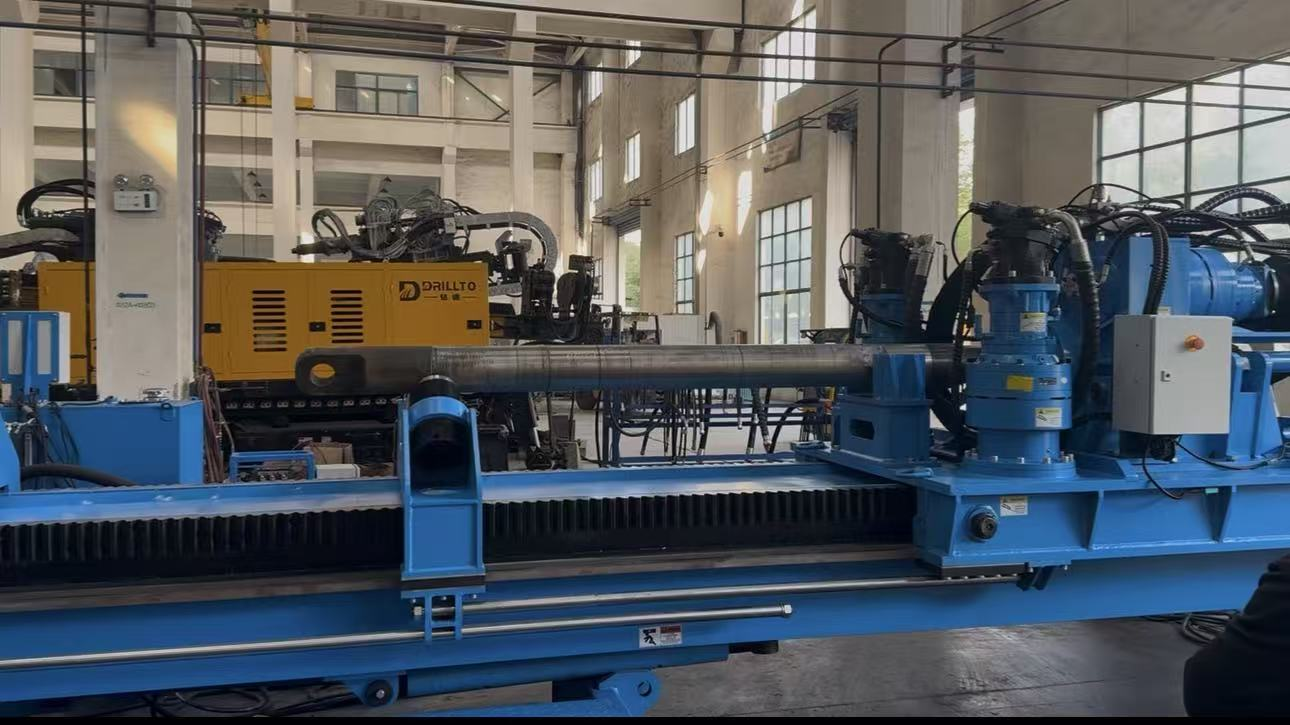
\includegraphics[width=145.000mm,height=0.76\textheight,keepaspectratio]{figure/research4-6/fig6-01-1.jpg}
\caption{井筒清洁工具评价实验装置实物}
\label{fig:r46-6-1}
\end{figure}

\begin{figure}[H]
\centering
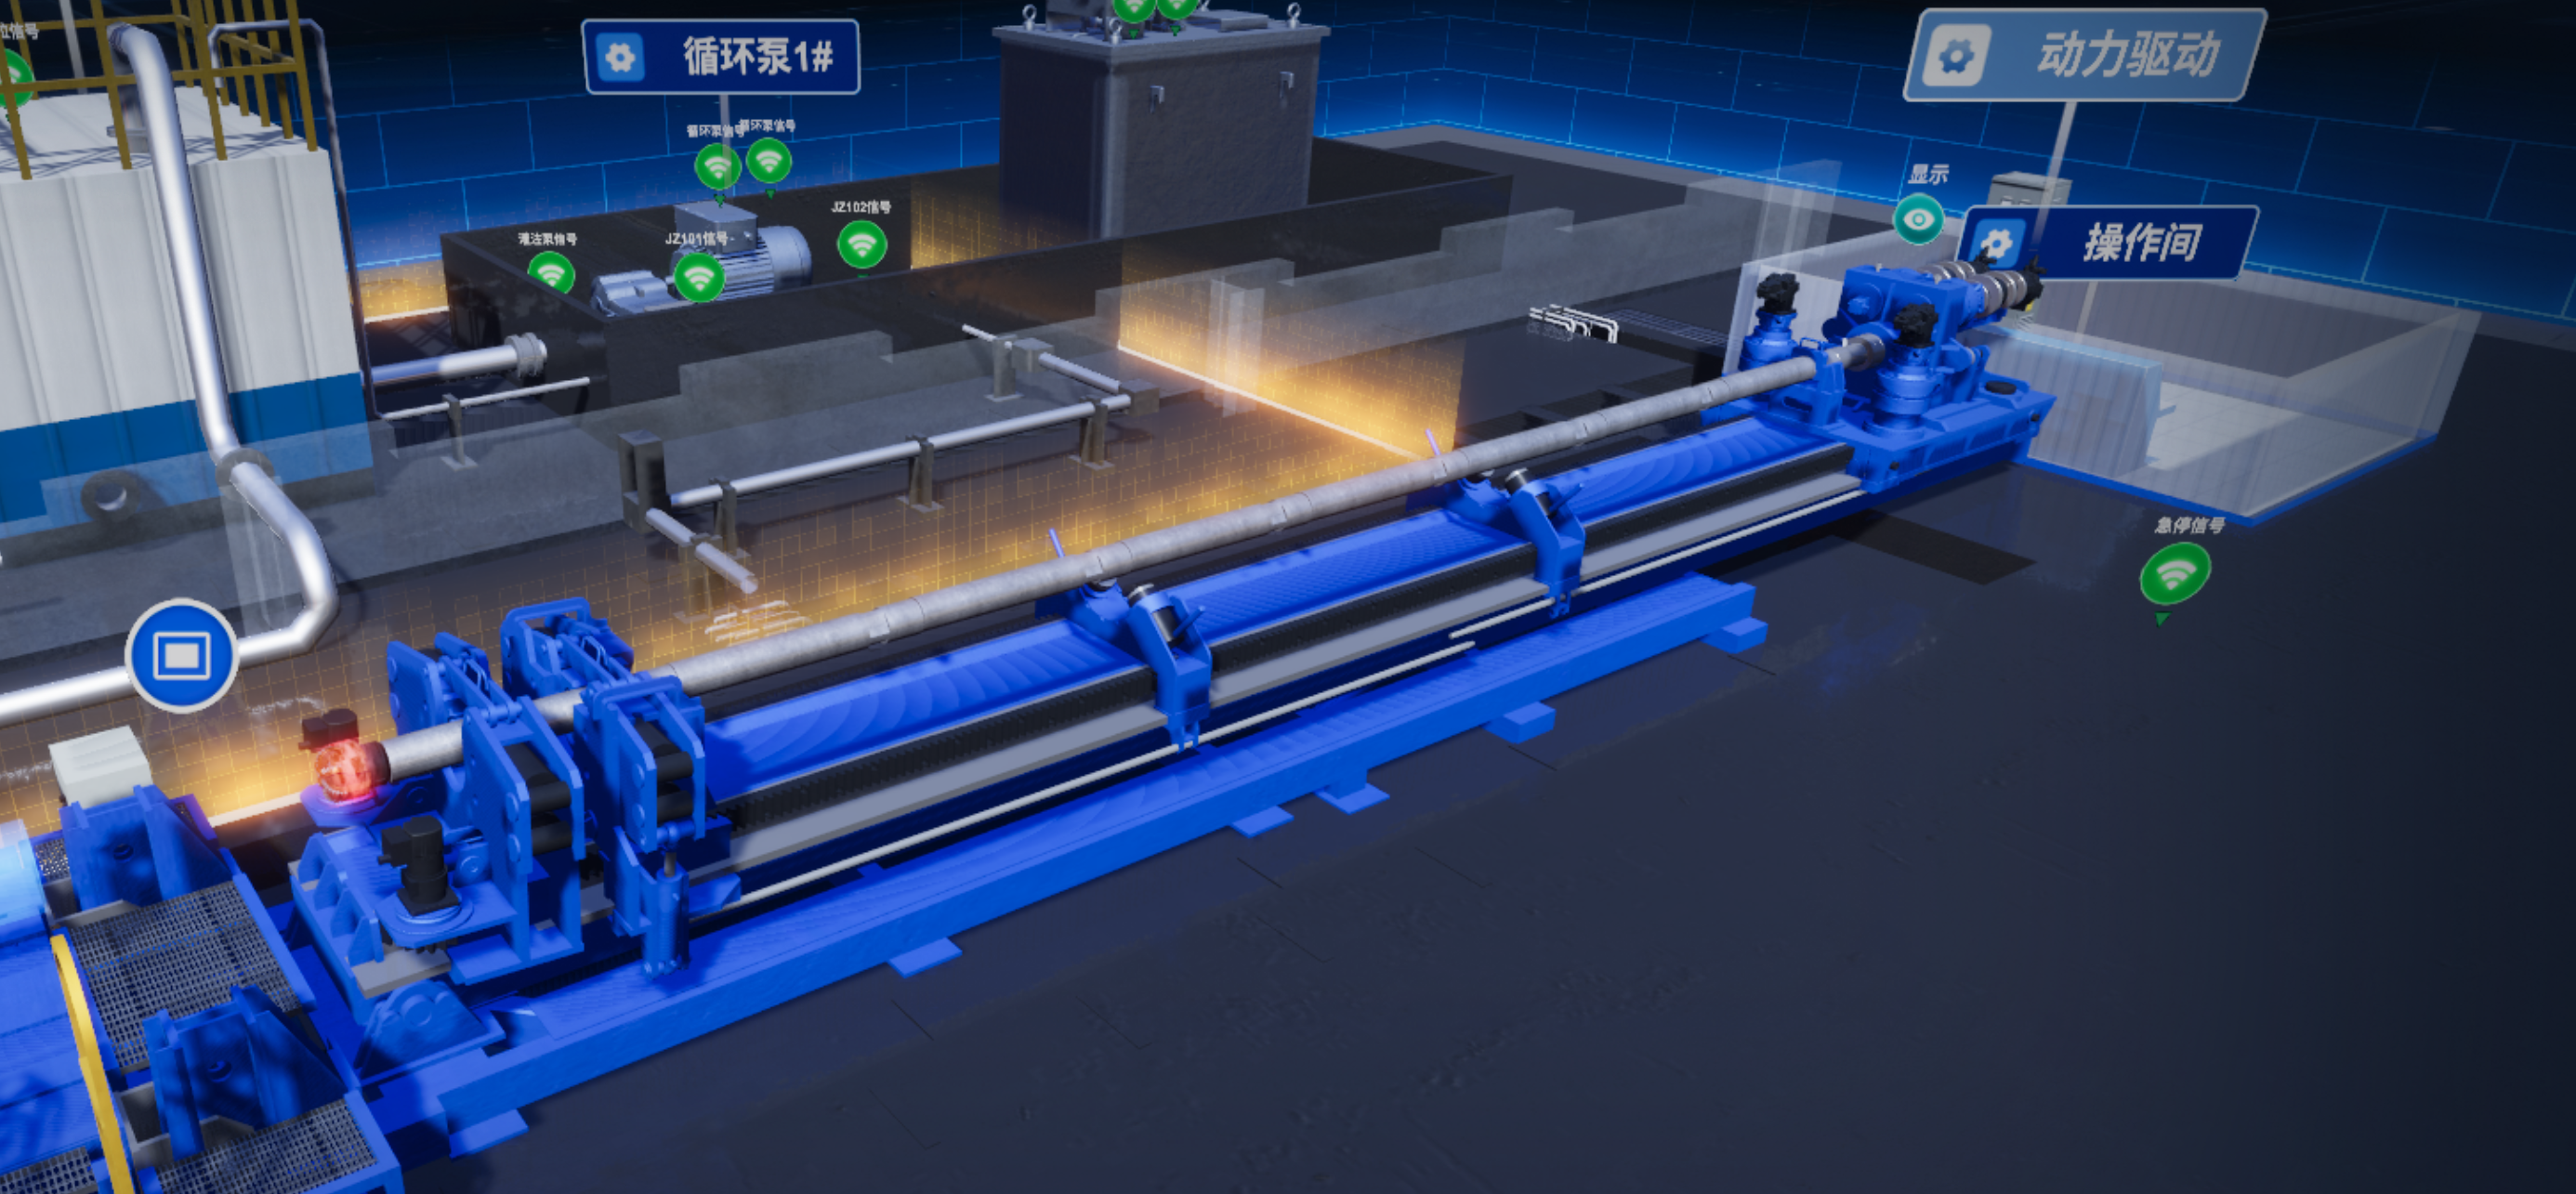
\includegraphics[width=145.000mm,height=0.76\textheight,keepaspectratio]{figure/research4-6/fig6-02-1.png}
\caption{评价实验装置数字孪生模型}
\label{fig:r46-6-2}
\end{figure}

轴向映射将设备位置对应到虚拟部件位置，旋转映射以主轴运动为对象更新模型状态。联调时核对运动方向、初始位置和停止状态，检查模型与装置在前进、停止、后退及旋转过程中的动作是否一致。三维场景中的设备标识与实际装置相对应，便于结合参数曲线定位正在运行的部件。

\section{运行数据接入与实验过程监测}
\label{sec:r46-6.3}

数字孪生应用完成室内部署，并与实验装置控制系统开展数据联调。实验界面以三维装置为主体，周边设置钻压、转速、扭矩、流量及位移等参数的数值或曲线显示。操作人员可在观察装置运动的同时查看参数变化，将加载、旋转和进给过程相互对应。

2026年9月30日现场联调中，控制端与孪生端的运行画面分别如图6-3、图6-4所示，记录了工具运行状态及对应参数。

\begin{figure}[H]
\centering
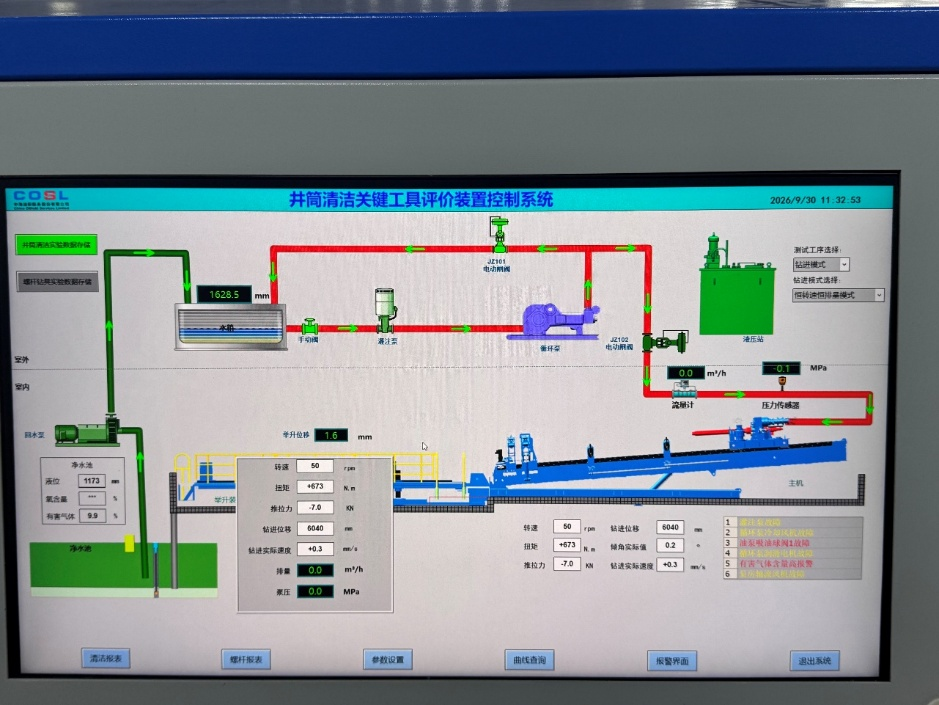
\includegraphics[width=120.000mm,height=0.76\textheight,keepaspectratio]{figure/research4-6/fig6-03-1.jpg}
\caption{现场联调中的评价装置控制界面}
\label{fig:r46-6-3}
\end{figure}

\begin{figure}[H]
\centering
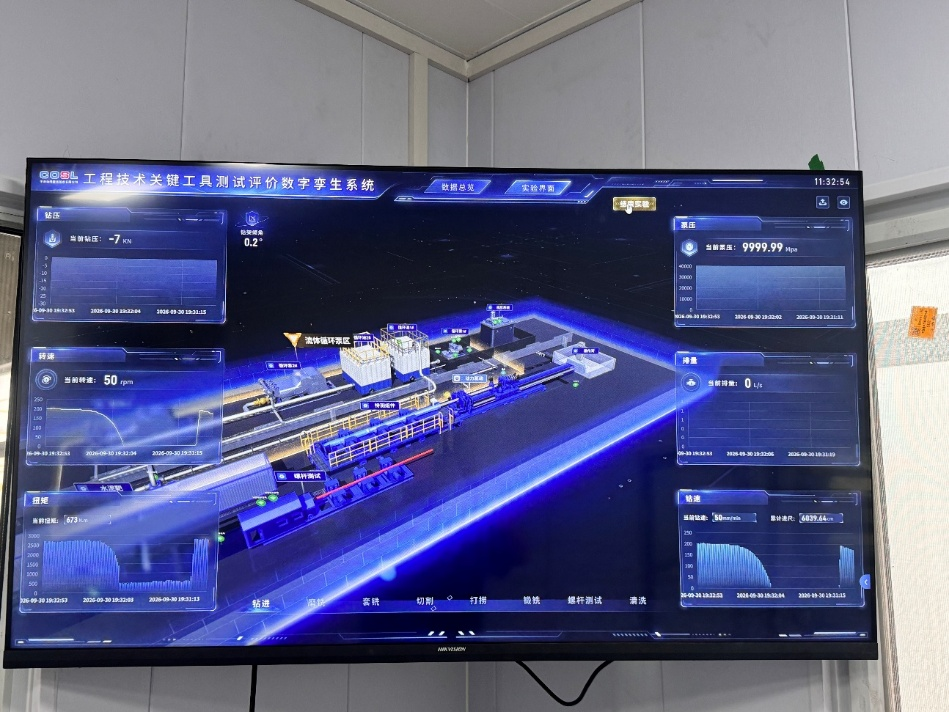
\includegraphics[width=120.000mm,height=0.76\textheight,keepaspectratio]{figure/research4-6/fig6-04-1.jpg}
\caption{现场联调中的数字孪生运行界面}
\label{fig:r46-6-4}
\end{figure}

\begin{table}[H]
\centering
\setstretch{1}
\fontsize{10.5}{15.75}\selectfont
\setlength{\tabcolsep}{3pt}
\renewcommand{\arraystretch}{1.1}
\arrayrulecolor{r46border}
\caption{现场联调画面的对应参数}\label{tab:r46-6-2}
\begin{tabular}{|>{\centering\arraybackslash}m{0.273979\dimexpr\linewidth-10\tabcolsep-6\arrayrulewidth\relax}|>{\centering\arraybackslash}m{0.184948\dimexpr\linewidth-10\tabcolsep-6\arrayrulewidth\relax}|>{\centering\arraybackslash}m{0.198599\dimexpr\linewidth-10\tabcolsep-6\arrayrulewidth\relax}|>{\centering\arraybackslash}m{0.157526\dimexpr\linewidth-10\tabcolsep-6\arrayrulewidth\relax}|>{\centering\arraybackslash}m{0.184948\dimexpr\linewidth-10\tabcolsep-6\arrayrulewidth\relax}|}
\hline
\rowcolor{r46gray} \textbf{核对参数} & \textbf{设备端} & \textbf{孪生端} & \textbf{绝对差值} & \textbf{数值一致度} \\ \hline
钻压/推拉力 & −7.0 kN & −7 kN & 0 kN & 100\% \\ \hline
转速 & 50 r/min & 50 r/min & 0 r/min & 100\% \\ \hline
位移/累计进尺 & 6040 mm & 6039.64 mm & 0.36 mm & 99.99404\% \\ \hline
\end{tabular}
\end{table}

控制端画面时间为2026年9月30日11\ensuremath{\mathbin{:}}32\ensuremath{\mathbin{:}}53，孪生端为11\ensuremath{\mathbin{:}}32\ensuremath{\mathbin{:}}54。表6-2按盖章说明附页统一单位：钻压与转速差值为0，位移差值为0.36 mm。以设备端数值为基准，相对偏差E=|孪生端值−设备端值|/|设备端值|×100\%，数值一致度S=max(0，100\%−E)，位移一致度为99.99404\%。

\section{系统联调与实验评价应用}
\label{sec:r46-6.4}

系统联调核对了工具前进、停止、后退和旋转动作，并比对控制端与孪生端的对应参数，形成实际装置照片、孪生运行画面和第三方盖章说明。上述成果支持评价实验运行数据驱动三维场景及参数显示的功能。

杭州多算科技有限公司于2026年10月8日出具的盖章说明确认，模型由实验数据驱动工具前进、后退和旋转，记录钻压、转速、位移，实现评价实验运转映射；附页列出的三项参数数值一致度均高于90\%。图6-5为签章说明，图6-6为参数比对及计算方法附页。参数数值比对用于核对两端显示，工作轨迹重合度结合实际与虚拟运动轨迹评价。

\begin{figure}[H]
\centering
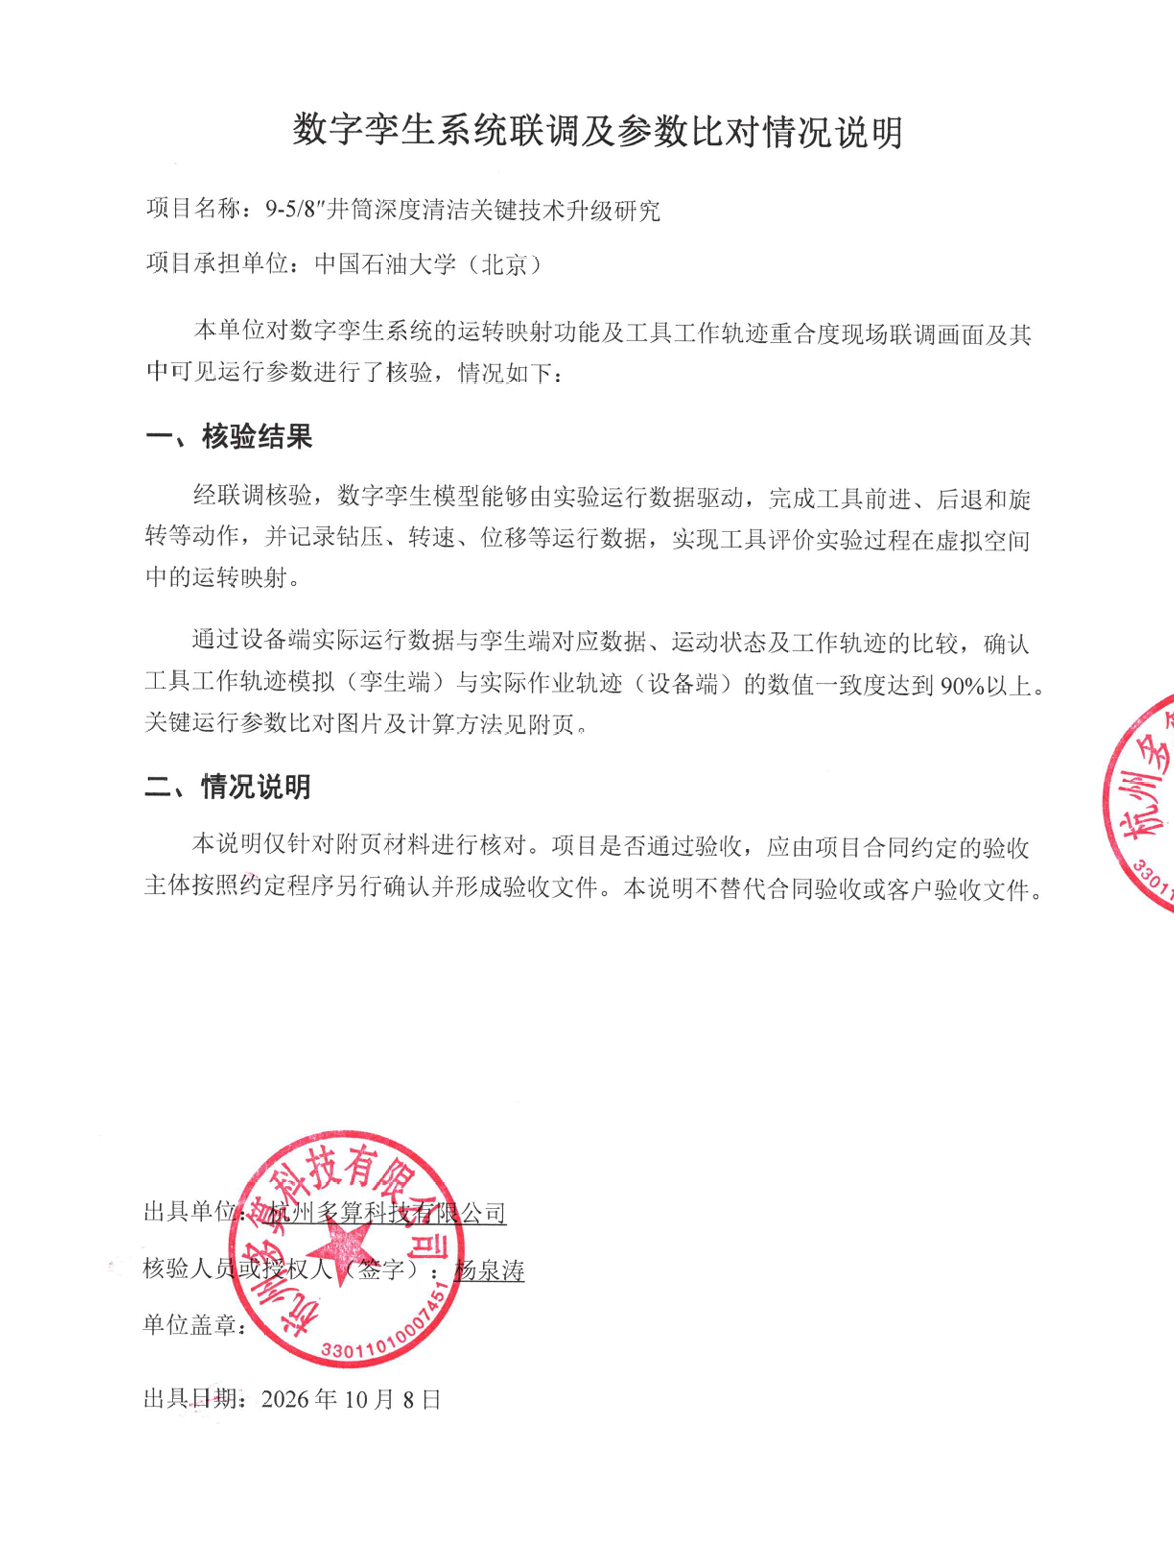
\includegraphics[width=126.107mm,height=0.76\textheight,keepaspectratio]{figure/research4-6/fig6-05-1.png}
\caption{数字孪生系统联调及参数比对签章说明}
\label{fig:r46-6-5}
\end{figure}

\begin{figure}[H]
\centering
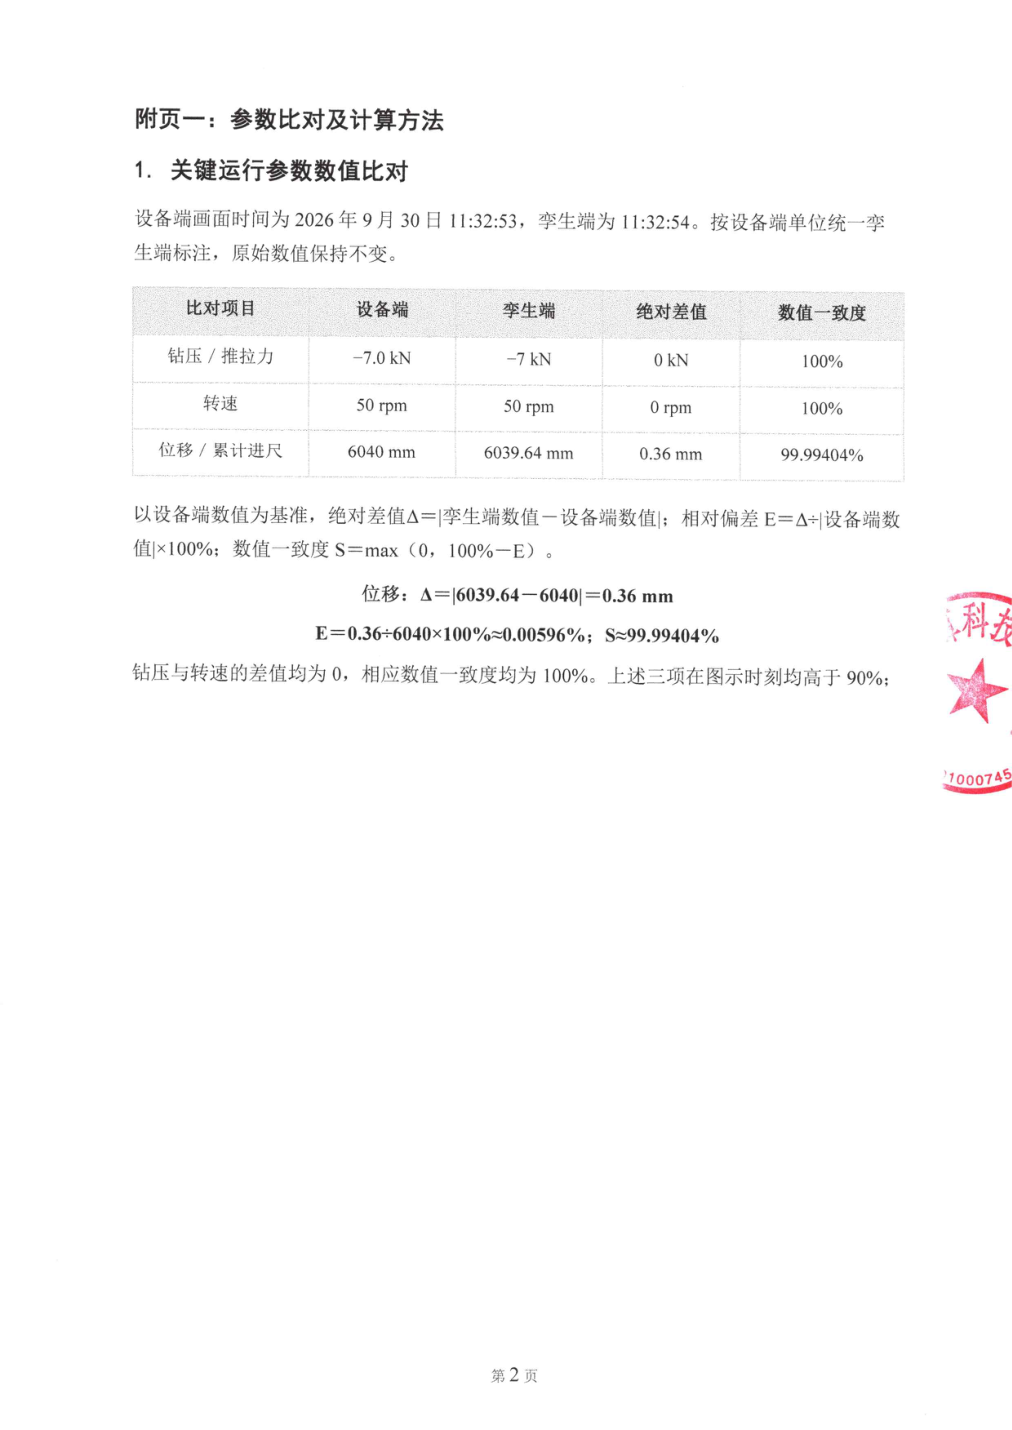
\includegraphics[width=117.000mm,height=0.76\textheight,keepaspectratio]{figure/research4-6/fig6-06-1.png}
\caption{盖章说明的参数比对及计算方法附页}
\label{fig:r46-6-6}
\end{figure}
